% \looseness=-1
\everypar{\looseness=-1}
\section{\approach Makes LLMs Better Agents}

In this section, we first describe \approach framework (\sref{sec:codeact_definition}) and provide empirical evidence that supports the choice of \approach.
% 
We focus on Python as the programming language for \approach due to its popularity (ranked top-1 at \cite{tiobe}) and numerous open-source packages. 
% 
We aim to answer several research questions (RQs) using 17 off-the-shelf LLMs. In \sref{sec:data-factor-format}, we examine RQ1: Does LLMs' familiarity with code due to a large amount of code pre-training data bring \approach advantages over text and JSON?
% 
We discuss RQ2 in \sref{sec:control-data-flow}: Does \approach benefit from Python’s innate control and data flow feature in complex problems?
% 
Finally, as an additional benefit, we discuss how using \approach further enhances LLM agents by enabling multi-turn interactions and allowing them to access existing software in \sref{sec:multiturn_software_benefit} and \fref{fig:qualitative_example}.

\begin{figure*}[!th]
    % \vspace{-10pt}
    \centering
    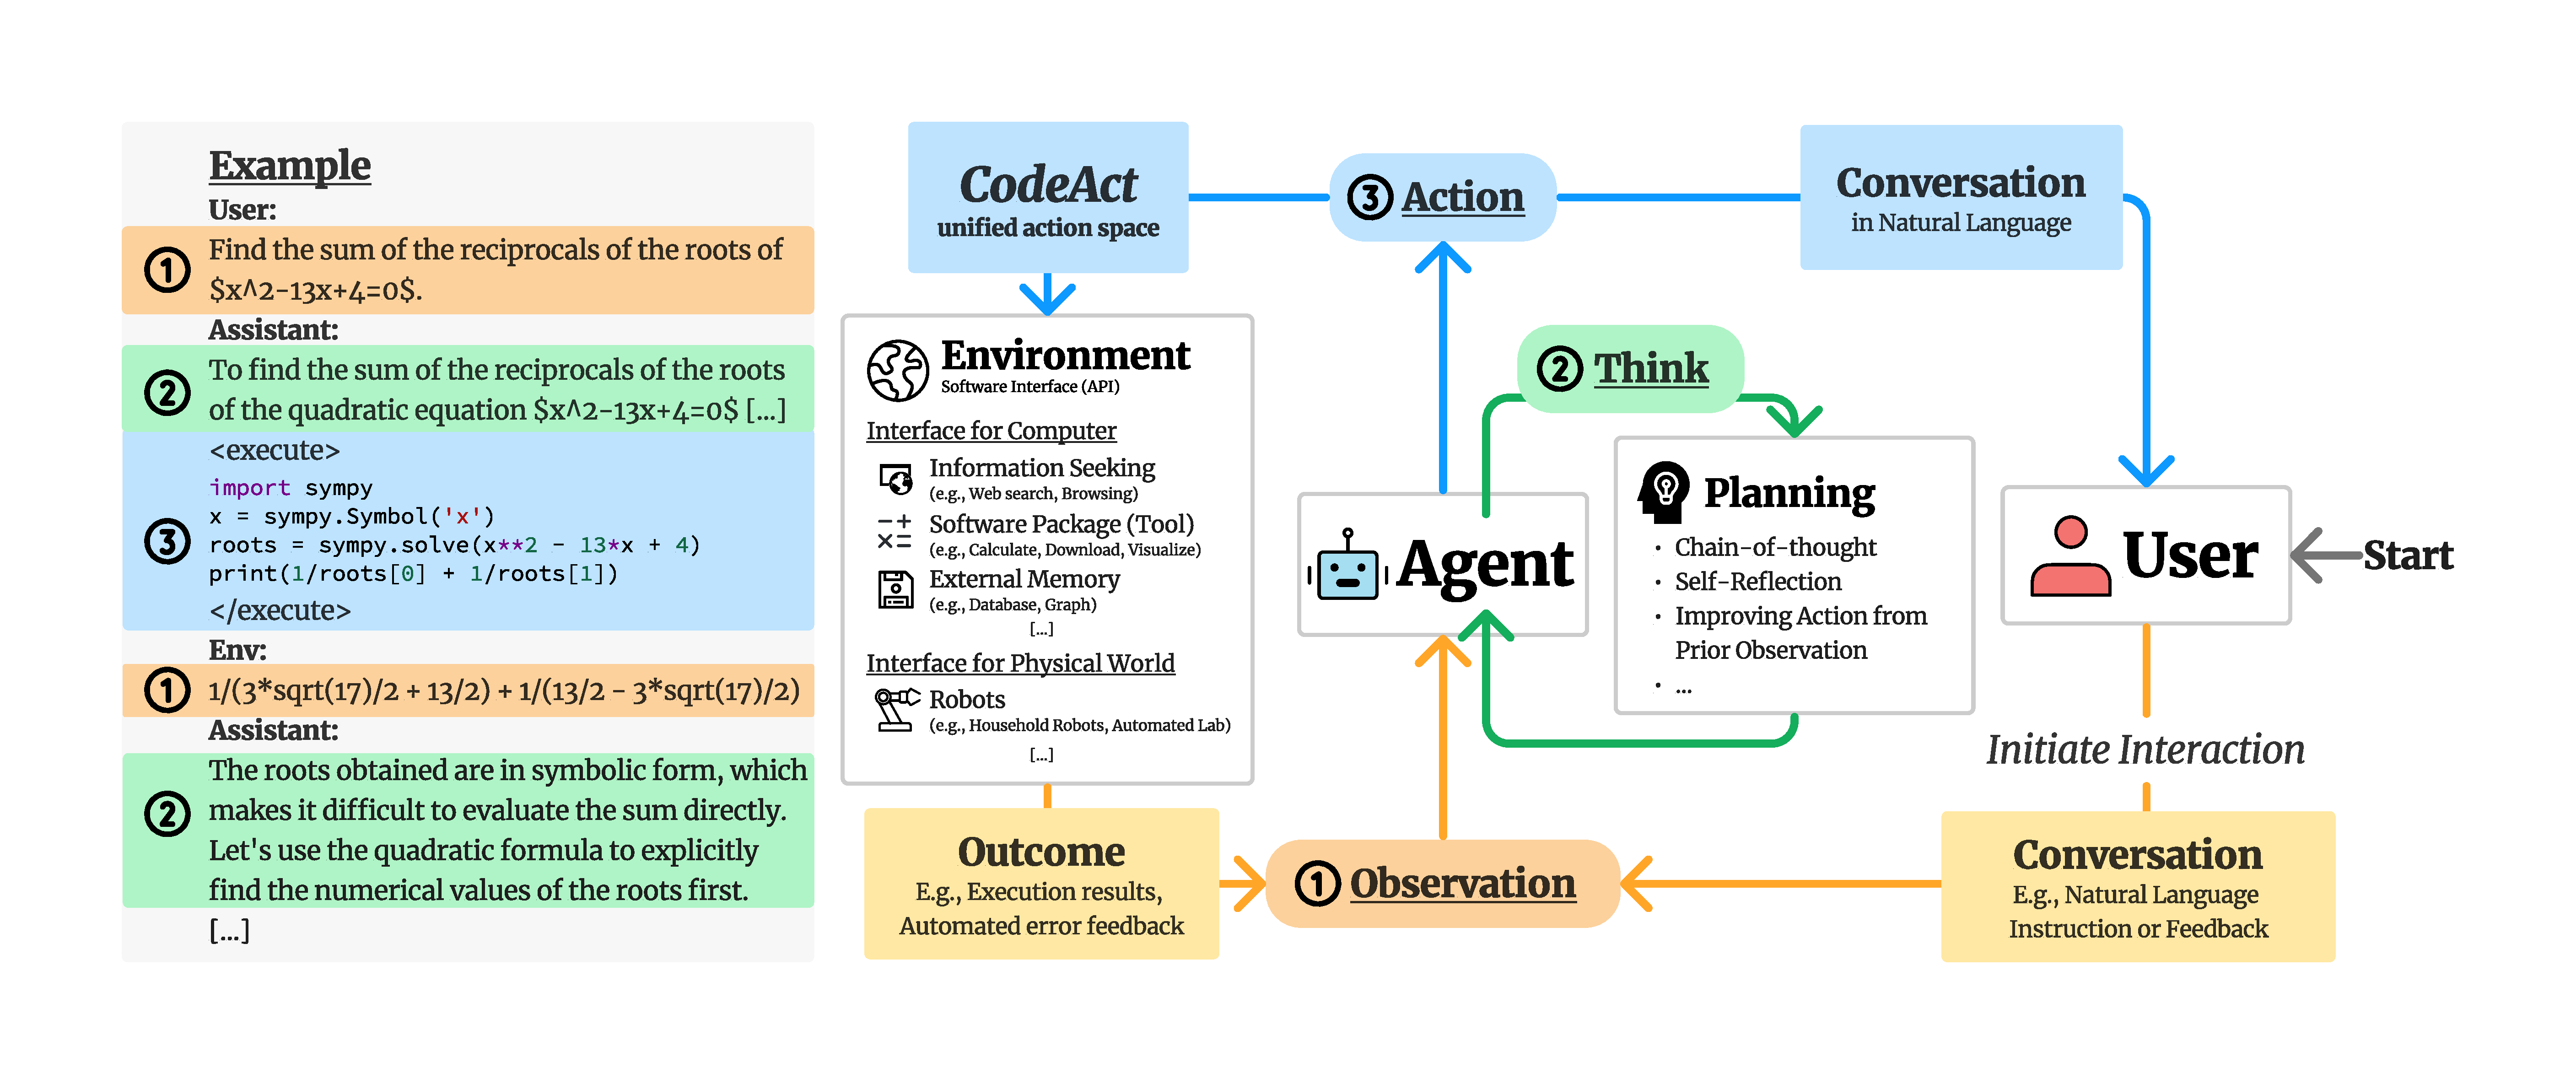
\includegraphics[width=\textwidth]{figures/codeactagent-data.pdf}
    \vspace{-20pt}
    % \vspace{-18pt}
    \caption{General agent multi-turn interaction framework that describes the role of \approach and motivates the construction of our data mixture. \dataname focuses on the \textit{agent-environment} interactions and specifically filters for the self-improved \textit{planning} behavior, while general conversation data we include focuses on \textit{agent-user} interaction (\sref{sec:agent_env_data}).
    }
    \label{fig:llm_agent_framework}
    % \vspace{-15pt}
\end{figure*}

\subsection{What is \approach?}
\label{sec:codeact_definition}

In \fref{fig:llm_agent_framework}, we first introduce a general multi-turn interaction framework for LLM agents' real-world usage that considers three roles \citep{yang2024unified}: \textit{agent}, \textit{user}, and \textit{environment}.
% 
We define \textit{interaction} as the information exchange between the agent and an external entity (user or environment).
% 
For each turn of interaction, the agent receives an \textit{observation} (input) either from the user (e.g., natural language instruction) or the environment (e.g., code execution result), optionally planning for its action through chain-of-thought \citep{wei2022chain}, and emits an \textit{action} (output) to either user in natural language or the environment.
% 
\approach employs Python code to consolidate all \textit{actions} for \textit{agent-environment interaction}. In \approach, each emitted \textit{action} to the environment is a piece of Python code, and the agent will receive outputs of code execution (e.g., results, errors) as \textit{observation}.
% 
We include an example prompt of \approach in \sref{sec:codeact_prompt}.


\subsection{\approach Shows the Promise as a Strong Tool Use Framework}
\label{sec:data-factor-format}
In this section, we perform a controlled experiment to understand which format (text, JSON, \approach) is more likely to lead an LLM to generate correct \textit{atomic} tool calls.
% 
The performance in this experiment reflects LLM's familiarity with the corresponding format.
We hypothesize that using \approach to call tools is a more natural way to use tools for the models, which typically have extensive exposure to \textit{code data} during their training.

\noindent \textbf{Setup.}
We re-purpose API-Bank \citep{li2023apibank} and test LLMs' API-calling performance, comparing \approach, JSON, and text actions.
% 
For each evaluation instance, we instruct LLM to generate \textit{one atomic} tool call in the format of a Python function call, JSON object, or text expression in a pre-defined format. A concrete example is shown in \tref{tab:apibank-action-example}.
% 
We use API-Bank's level-1 instructions and the provided toolset. To evaluate API-calling, we follow their \textit{correctness} metric, matching the ground-truth API outputs with the actual model-generated API's execution outputs.

\noindent \textbf{Results.}
We present results in \tref{tab:api-bank-results}. 
% 
For most LLMs, \approach achieves comparable or better performance even in atomic actions (the simplistic tool use scenario) where its control and data flow strengths are ablated.
% 
Compared to closed-source LLMs, \approach's improvements are more prominent in open-source models. Furthermore, code data is usually more accessible for fine-tuning open-source LLMs than the specialized JSON or text tool-calling format.
% 
Although JSON is consistently weaker than other approaches for open-source models, it achieves decent performance with closed-source LLMs, indicating that these closed-source models may have gone through targeted fine-tuning toward their JSON capabilities.
% 
These results suggest optimizing for \approach is a better route for open-source LLMs than alternatives to improve their tool-use capabilities, as they already show good initial \approach capability due to extensive exposure to code data during pre-training.

\begin{table*}[bpth]
% \vspace{-15pt}
\begin{minipage}{0.40\textwidth}
\centering
\caption{
% \citep{li2023apibank}
Atomic API call correctness on API-Bank.
The best performance is \textbf{bolded}, and the second-best is \underline{underlined}.
}
\vspace{-5pt}
\label{tab:api-bank-results}
\begin{adjustbox}{max width=\textwidth}
\begin{tabular}{@{} l rrr @{}}
\toprule
& \multicolumn{3}{c}{\textbf{Correctness} (\%, $\uparrow$)} \\
\textbf{Format of Action} &  \approach &  JSON &  Text \\
\midrule
\multicolumn{4}{c}{\textit{Open-source LLMs}} \\

\texttt{CodeLlama-7b-Instruct-hf}  &  \underline{$12.5$} &              $12.0$ &     $\mathbf{17.0}$ \\
\texttt{CodeLlama-13b-Instruct-hf} &  \underline{$11.8$} &               $7.8$ &     $\mathbf{14.0}$ \\
\texttt{CodeLlama-34b-Instruct-hf} &     $\mathbf{17.3}$ &              $12.0$ &  \underline{$16.8$} \\
\texttt{Llama-2-7b-chat-hf}        &     $\mathbf{28.8}$ &              $11.3$ &  \underline{$25.8$} \\
\texttt{Llama-2-13b-chat-hf}       &     $\mathbf{38.1}$ &               $8.5$ &  \underline{$37.3$} \\
\texttt{Llama-2-70b-chat-hf}       &  \underline{$35.6$} &              $14.3$ &     $\mathbf{37.6}$ \\
\texttt{Mistral-7B-Instruct-v0.1}  &   \underline{$2.5$} &               $2.3$ &      $\mathbf{3.0}$ \\
\texttt{lemur-70b-chat-v1}         &     $\mathbf{58.6}$ &              $46.6$ &  \underline{$56.1$} \\

\midrule
\multicolumn{4}{c}{\textit{Closed-source LLMs}} \\

\texttt{claude-2}                  &     $\mathbf{76.7}$ &              $59.4$ &  \underline{$73.7$} \\
\texttt{claude-instant-1}          &     $\mathbf{75.2}$ &              $64.9$ &  \underline{$73.2$} \\
\texttt{gemini-pro}                &              $70.4$ &     $\mathbf{73.2}$ &  \underline{$71.2$} \\
\texttt{gpt-3.5-turbo-0613}        &     $\mathbf{74.4}$ &  \underline{$73.9$} &              $73.4$ \\
\texttt{gpt-3.5-turbo-1106}        &  \underline{$75.4$} &     $\mathbf{78.4}$ &              $73.4$ \\
\texttt{gpt-4-0613}                &  \underline{$75.4$} &     $\mathbf{82.0}$ &              $74.4$ \\
\texttt{gpt-4-1106-preview}        &  \underline{$76.7$} &     $\mathbf{82.7}$ &              $73.4$ \\
\texttt{text-davinci-002}          &     $\mathbf{69.2}$ &  \underline{$59.6$} &              $57.4$ \\
\texttt{text-davinci-003}          &  \underline{$75.4$} &     $\mathbf{76.9}$ &              $69.7$ \\
\midrule

\multicolumn{4}{c}{\textbf{Frequency of Best-Performing Format} $\uparrow$} \\
Open-source & $\mathbf{4}$ & $0$ & \underline{$4$} \\
Closed-source & \underline{$4$} & $\mathbf{5}$ & $0$ \\
\textbf{Overall} & $\mathbf{8}$ & $\underline{5}$ & $4$ \\
\bottomrule
\end{tabular}
\end{adjustbox}

\end{minipage}\hfill%
\begin{minipage}{0.58\textwidth}
\centering
\caption{Success rates (higher the better) and average turns required per instance (lower the better) on \evalname. The best results for each model are \textbf{bolded}, and the second-best ones are \underline{underlined}.
}
\vspace{-5pt}
\label{tab:zeroshot_act_results}
\begin{adjustbox}{max width=\textwidth}
\begin{tabular}{@{} l rrr  m{0.01em}  rrr @{}}
\toprule
{} & \multicolumn{3}{c}{\textbf{Success Rate (\%, $\uparrow$)}} && \multicolumn{3}{c}{\textbf{Avg. Turns} ($\downarrow$)} \\
\cmidrule{2-4}
\cmidrule{6-8}

\textbf{Format of Action} & \approach & JSON & Text && \approach & JSON & Text \\

\midrule

\multicolumn{8}{c}{\textit{Open-source LLMs}} \\

\texttt{CodeLlama-7b-Instruct-hf}  &      $\mathbf{4.9}$ &   \underline{$2.4$} &   \underline{$2.4$} &&     $\mathbf{9.7}$ &   \underline{$9.9$} &   \underline{$9.9$} \\
\texttt{CodeLlama-13b-Instruct-hf} &      $\mathbf{4.9}$ &      $\mathbf{4.9}$ &      $\mathbf{4.9}$ &&  \underline{$9.8$} &   \underline{$9.8$} &      $\mathbf{9.7}$ \\
\texttt{CodeLlama-34b-Instruct-hf} &      $\mathbf{2.4}$ &   \underline{$0.0$} &   \underline{$0.0$} &&     $\mathbf{9.9}$ &  \underline{$10.0$} &  \underline{$10.0$} \\
\texttt{Llama-2-7b-chat-hf}        &               $0.0$ &   \underline{$1.2$} &      $\mathbf{2.4}$ &&     $\mathbf{8.9}$ &   \underline{$9.5$} &               $9.6$ \\
\texttt{Llama-2-13b-chat-hf}       &      $\mathbf{0.0}$ &      $\mathbf{0.0}$ &      $\mathbf{0.0}$ &&     $\mathbf{9.7}$ &  \underline{$10.0$} &  \underline{$10.0$} \\
\texttt{Llama-2-70b-chat-hf}       &     $\mathbf{11.0}$ &   \underline{$3.7$} &   \underline{$3.7$} &&     $\mathbf{9.1}$ &   \underline{$9.8$} &   \underline{$9.8$} \\
\texttt{Mistral-7B-Instruct-v0.1}  &               $0.0$ &      $\mathbf{3.7}$ &   \underline{$1.2$} &&             $10.0$ &      $\mathbf{9.8}$ &   \underline{$9.9$} \\
\texttt{lemur-70b-chat-v1}         &  \underline{$13.4$} &     $\mathbf{15.9}$ &              $12.2$ &&     $\mathbf{9.1}$ &   \underline{$9.3$} &               $9.4$ \\

\midrule 
\multicolumn{8}{c}{\textit{Closed-source LLMs}} \\

\texttt{claude-2}                  &     $\mathbf{54.9}$ &  \underline{$39.0$} &              $29.3$ &&     $\mathbf{7.2}$ &   \underline{$8.3$} &               $8.5$ \\
\texttt{claude-instant-1}          &              $20.7$ &     $\mathbf{31.7}$ &  \underline{$24.4$} &&  \underline{$8.8$} &      $\mathbf{8.6}$ &               $8.9$ \\
\texttt{gemini-pro}                &     $\mathbf{22.0}$ &  \underline{$19.5$} &              $11.0$ &&     $\mathbf{8.8}$ &   \underline{$9.1$} &               $9.5$ \\
\texttt{gpt-3.5-turbo-0613}        &     $\mathbf{51.2}$ &  \underline{$26.8$} &              $20.7$ &&     $\mathbf{7.0}$ &   \underline{$8.8$} &               $9.2$ \\
\texttt{gpt-3.5-turbo-1106}        &     $\mathbf{29.3}$ &  \underline{$15.9$} &              $14.6$ &&     $\mathbf{8.4}$ &   \underline{$9.0$} &   \underline{$9.0$} \\
\texttt{gpt-4-0613}                &     $\mathbf{67.1}$ &  \underline{$56.1$} &              $45.1$ &&     $\mathbf{6.6}$ &   \underline{$7.6$} &               $8.0$ \\
\texttt{gpt-4-1106-preview}        &     $\mathbf{74.4}$ &              $52.4$ &  \underline{$53.7$} &&     $\mathbf{5.5}$ &   \underline{$7.6$} &               $7.7$ \\
\texttt{text-davinci-002}          &   \underline{$4.9$} &   \underline{$4.9$} &      $\mathbf{8.5}$ &&  \underline{$9.7$} &               $9.8$ &      $\mathbf{9.6}$ \\
\texttt{text-davinci-003}          &     $\mathbf{20.7}$ &  \underline{$18.3$} &               $7.3$ &&  \underline{$9.2$} &      $\mathbf{9.0}$ &               $9.6$ \\

\midrule
\multicolumn{7}{c}{\textbf{Frequency of Best-performing Format} $\uparrow$} \\
Open-source & $\mathbf{5}$ & \underline{$4$} & $3$ && $\mathbf{6}$ & \underline{$1$} & \underline{$1$} \\

Closed-source & $\mathbf{7}$ & \underline{$1$} & \underline{$1$} && $\mathbf{6}$ & \underline{$2$} & $1$ \\

\textbf{Overall} & $\mathbf{12}$ & \underline{5} & $4$ && $\mathbf{12}$ &  \underline{$3$} & $2$ \\


\bottomrule
\end{tabular}
\end{adjustbox}
\end{minipage}
% \vspace{-15pt}
\end{table*}



\subsection{\approach Gets More Done with Fewer Interactions}
\label{sec:control-data-flow}


In this section, we investigate whether LLM agents can benefit from the control and data flow of code on problems that require complex patterns of tool use.

\noindent \textbf{\evalname.}
As shown in \tref{tab:tool_bench_comparison}, to the best of our knowledge, no existing tool-use benchmarks contain complex tasks requiring the composition of multiple tools while supporting evaluating different action formats. Hence, we curate a benchmark \evalname to fill this gap, which evaluates LLMs' capabilities in solving complex tasks that typically require \textbf{m}ultiple calls to \textbf{m}ultiple tools in \textbf{m}ulti-turn interactions.
% 
It contains 82 human-curated instances, spanning tasks including web browsing, finance, travel itinerary planning, science, and information processing. 
% 
Each domain is accompanied by a unique set of manually crafted tools.
%
We intentionally keep the prompt simple (examples in \sref{sec:zeroshot_act_prompt}) and avoid providing any demonstration to test the LLM's zero-shot ability to use tools, similar to how a novice user without knowledge of few-shot prompting would use the model.
% 
% Please refer to \sref{sec:zeroshot_act_prompt} for prompt examples.

\noindent \textbf{Setup.}
We allow the model to generate fully functional Python code that enables control and data flow (e.g., if-statement, for-loop). We follow the action format for JSON and text described in \tref{tab:apibank-action-example}.
% 
Within each turn, the model can either emit an \textit{action} or propose an \textit{answer} to be verified by an exact match with the ground-truth solution.
The interaction will terminate when a maximum of 10 interaction turns are reached or a correct solution has been submitted, similar to \cite{wang2023mint}.

\noindent \textbf{Metric.} We measure the \textit{success rate} by calculating the percentage of the model proposed answers that match the ground-truth solutions. We also include the \textit{avg. turns} metric: the average number of turns on all evaluated instances.

\noindent \textbf{Quantitative Results on \evalname.}
We include full results in \tref{tab:zeroshot_act_results} and a subset of results for visualization in \fref{fig:zeroshot_acteval}.
% 
\approach generally has a higher task success rate (12 out of 17 evaluated LLMs), similar to the trend in \sref{sec:data-factor-format}. Moreover, using \approach requires a lower average number of turns (12 out of 17 evaluated LLMs).
% 
For example, the best model \texttt{gpt-4-1106-preview} achieves a $20.7$\% absolute improvement compared to the next best action format (text) while requiring $2.1$ fewer interaction turns on average.
%
However, there is still a significant gap in terms of absolute \approach performance between open- and closed-source LLMs as the best open-source model achieving 13.4\% while the best closed-source model \texttt{gpt-4-1106-preview} 74.4\%. This is potentially due to open-source models' weak task-solving capability and inability to follow complex instructions without demonstration, suggesting an urgent need to improve open-source LLMs for practical, real-world tasks under the zero-shot setting.

\begin{figure*}[!ht]
    \centering
    % 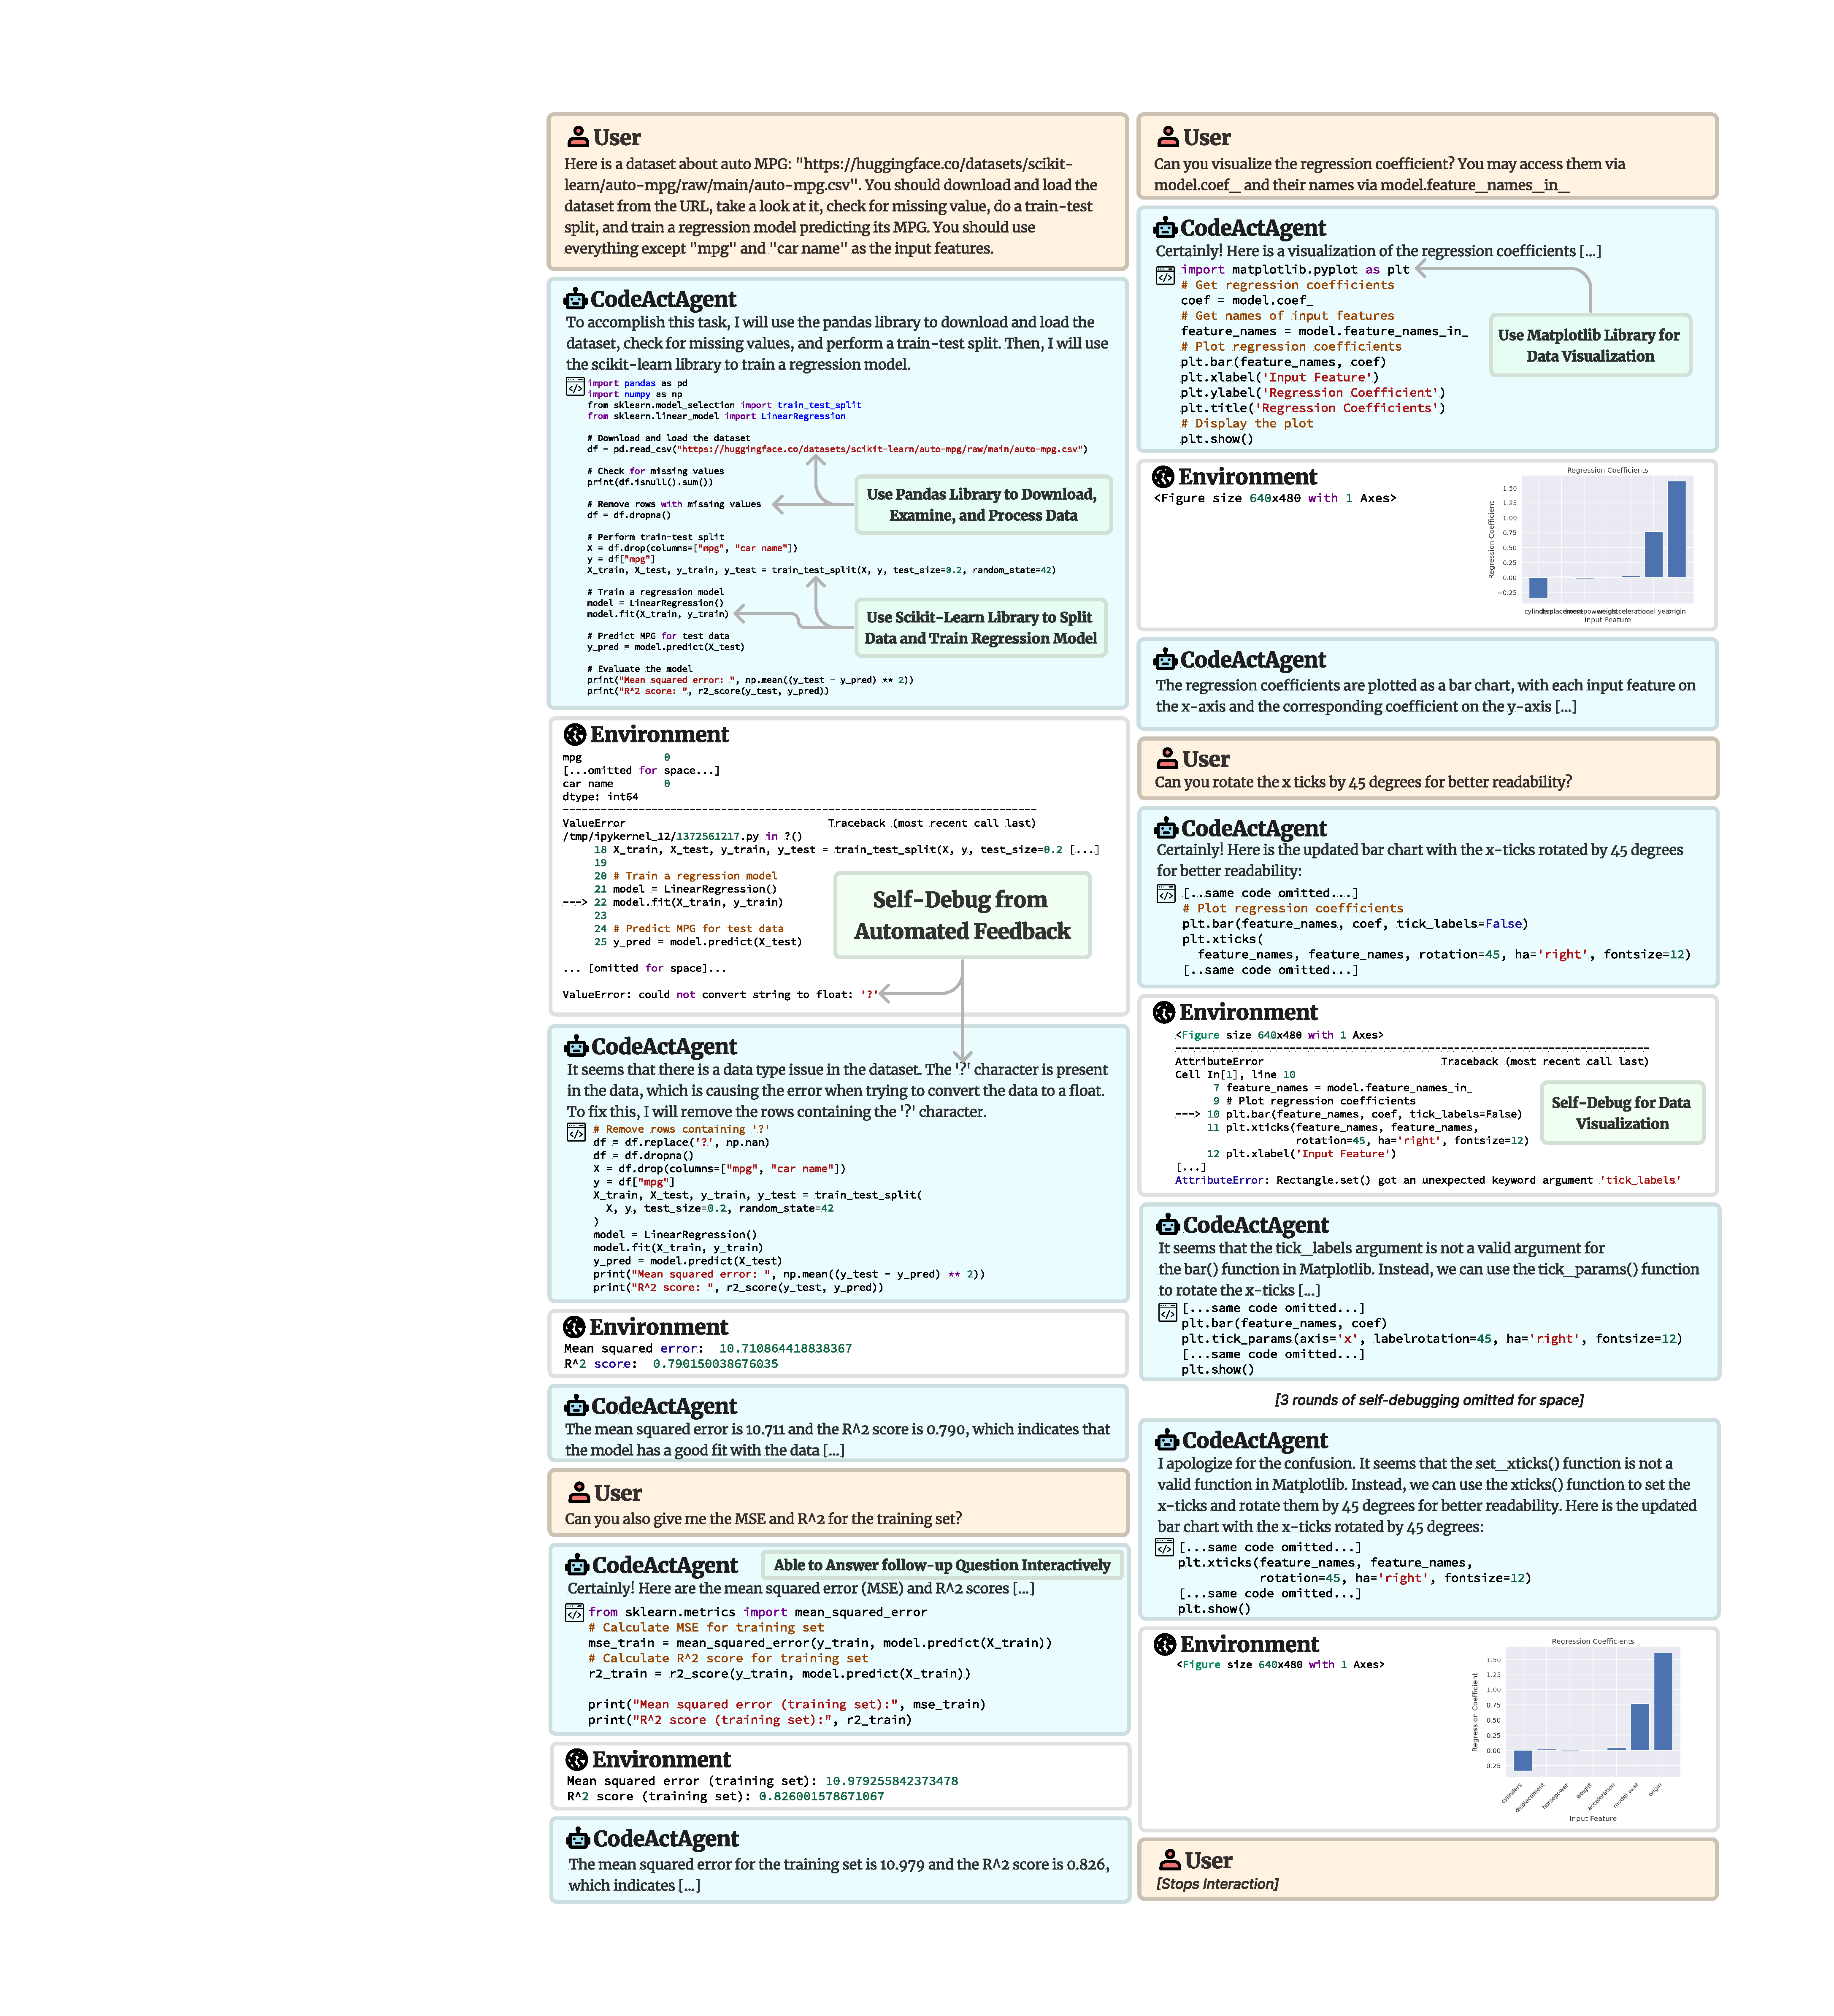
\includegraphics[width=\textwidth]{figures/codeactagent-qualitative-succint-2col.pdf}
    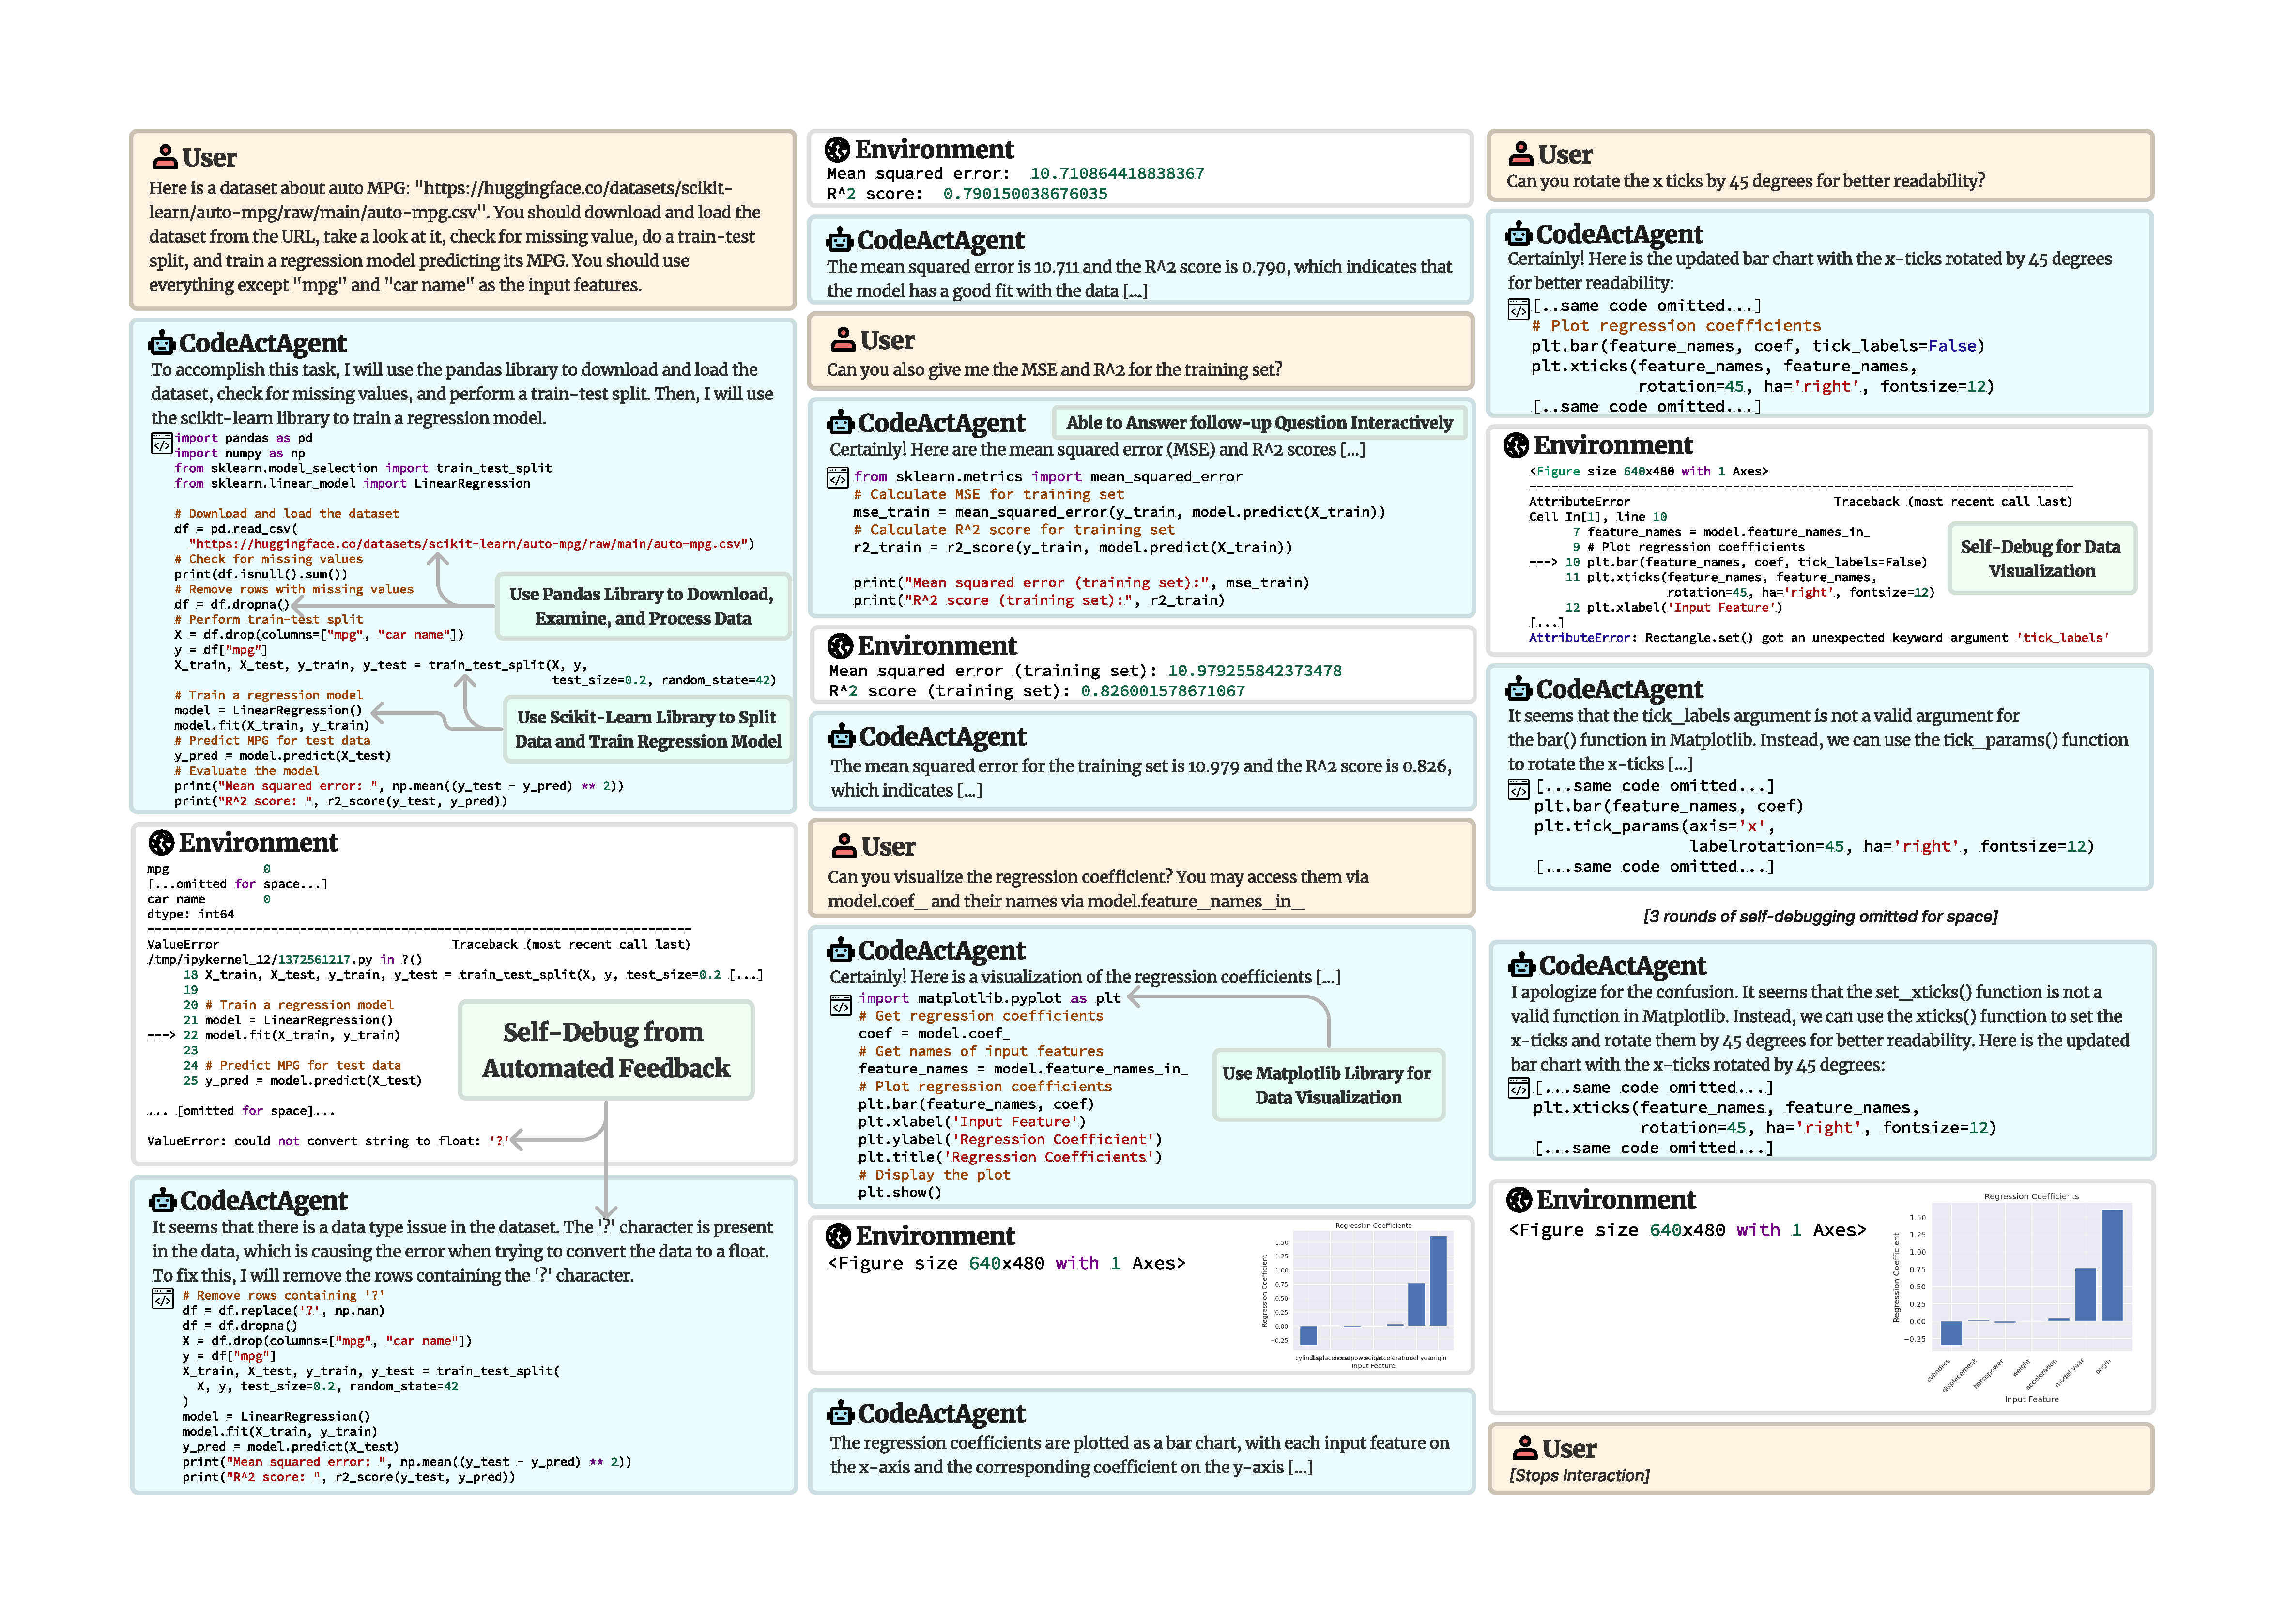
\includegraphics[width=\textwidth]{figures/codeactagent-qualitative-succint-3col.pdf}
    \vspace{-20pt}
    \caption{Example multi-turn interaction with Python packages using \modelname (Mistral-7b). No in-context demonstrations are provided to the model. Some messages are omitted for space.
    See \url{https://chat.xwang.dev/r/Vqn108G} for complete interaction.
    }
    \label{fig:qualitative_example}
\end{figure*}


\subsection{\approach Benefits from Multi-turn Interactions and Existing Software Packages}
\label{sec:multiturn_software_benefit}

In \fref{fig:qualitative_example}, we show how an LLM agent can integrate with Python (i.e., \modelname we trained in \sref{sec:llm_agent_evaluation}) and use existing software to perform complex tasks in multi-turn interactions.
%
Thanks to its extensive knowledge of Python learned during pre-training, the LLM agent can automatically import the correct \textit{Python libraries} to solve tasks without requiring user-provided tools or demonstrations.
% 
As illustrated in \fref{fig:qualitative_example}, \modelname can use Pandas to download and process tabular data, use Scikit-Learn for machine learning train-test data split and regression model training, and use Matplotlib for data visualization.
% 
Furthermore, using the interactive Python interpreter for code execution allows automated error messages that help the LLM agent `self-debug' their actions in a \textit{multi-turn interaction} and eventually complete the human user's request correctly.

